\section{扭转的概念}
\vspace*{-1.5em}
\begin{definition}[扭转变形]
	扭转变形是杆件受到大小相等,方向相反且作用平面垂直于杆件轴线的力偶作用,使杆件的横截面绕轴线产生转动。
	\begin{itemize}
		\item 受力特点
		\par 杆件的两端作用两个\md{大小相等}、\md{方向相反}、且\md{作用面垂直于杆件轴线}的力偶.
		\item 变形特点
		\par 杆件的任意两个横截面都发生绕轴线的相对转动.
	\end{itemize}
	\end{definition}

\section{外力偶矩的计算}
\vspace*{-1.5em}
\begin{theorem}[外力偶矩]
	工程中有许多传递功率的轴,需要根据它的转速$n$和传递的功率$N_p$计算出外力偶矩。力偶在单位时间内所作之功就是功率,它等于:
\begin{equation}
	N_p = M_n \omega
\end{equation}
$N_p$常用$\text{kw}$(千瓦)表示,而$w$常用$\text{rpm}$(转/分)表示.即
\margin{\\$M_\text{e}$ \quad 外力偶矩($\text{N}/\text{m}$)\\$P$ \quad 功率($\text{kw}$)\\$n$ \quad 转速($\text{r/min}$)}
\begin{equation}
	M_\text{e}=9549\,\frac{P}{n}
\end{equation}
\end{theorem}

\section{扭矩和扭矩图}
\subsection{扭矩的计算}

\smallboxa[截面法]{JMF} 求内力时,在$n-n$截面处假想将轴截开取左侧为研究对象,由
$$
\sum M_x = 0
$$
可以得到
\begin{equation}
	T=M_\text{e}
\end{equation}
其中$T$就称为\md{扭矩}.(参看图\ref{扭矩1}和图\ref{扭矩2})

\begin{figure}[!htbp]
	\centering
	
	\subfigure[扭转总体图]{
		\begin{minipage}[t]{0.5\linewidth}
			\centering
			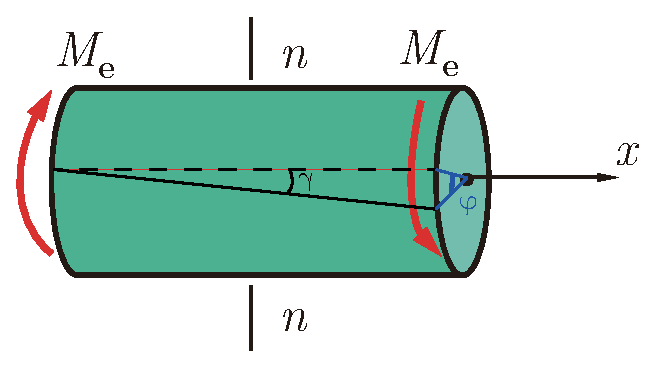
\includegraphics[width=0.9\linewidth]{picture/p2_c3/扭矩和扭矩图_1.eps}
			\label{扭矩1}
		\end{minipage}%
	}%
	\subfigure[扭矩图]{
		\begin{minipage}[t]{0.5\linewidth}
			\centering
			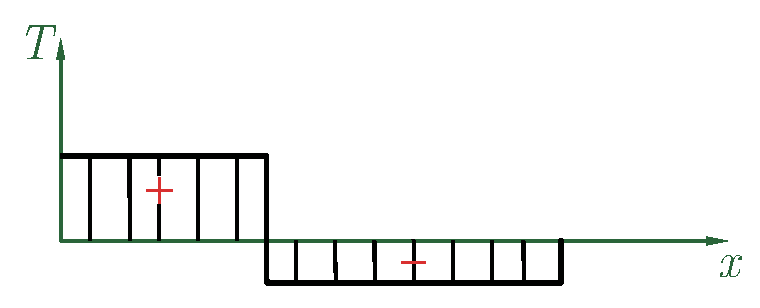
\includegraphics[width=0.9\linewidth]{picture/p2_c3/扭矩和扭矩图_4.eps}
			\label{扭矩4}
		\end{minipage}%
	}%

	%这个回车键很重要 \quad也可以
	\subfigure[截面左侧]{
		\begin{minipage}[t]{0.5\linewidth}
			\centering
			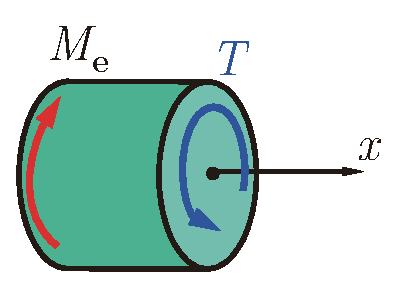
\includegraphics[width=0.7\linewidth]{picture/p2_c3/扭矩和扭矩图_2.eps}
			\label{扭矩2}
		\end{minipage}
	}%
	\subfigure[截面右侧]{
		\begin{minipage}[t]{0.5\linewidth}
			\centering
			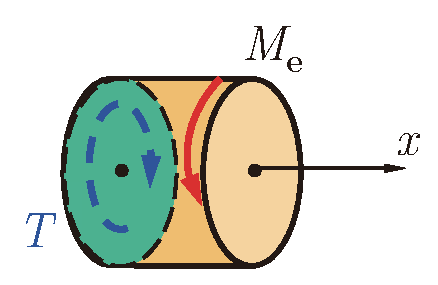
\includegraphics[width=0.75\linewidth]{picture/p2_c3/扭矩和扭矩图_3.eps}
			\label{扭矩3}
		\end{minipage}
	}%
	
	\centering
	\caption{扭矩与扭矩图}
\end{figure}

\subsection{扭矩的符号规定}
采用右手螺旋法则,当力偶矩矢的指向背离截面时扭矩为正,反之为负.

\subsection{扭矩图}
用平行于杆轴线的坐标 $x$ 表示横截面的位置;用垂直于杆轴线的坐标 $T$ 表示横截面上的扭矩,正的扭矩画在 $x$ 轴上方,负的扭矩画在 $x$轴下方.(参看图\ref{扭矩4})

\section{纯剪切}
\subsection{薄壁圆筒扭转}
\vspace{0.5em}
\smallboxb[受力特点]
	\begin{itemize}
	\item 横截面上无正应力,只有切应力;
	\item 切应力方向垂直半径或与圆周相切.
\end{itemize}
圆周各点处切应力的方向于圆周相切,且数值相等,近似的认为沿壁厚方向各点处切应力的数值无变化.

\begin{theorem}[薄壁圆筒扭转时的切应力]
	由扭矩$T$的定义,有
	\margin{\\ $T$ \quad 扭矩(N/m)\\ $\tau$ \quad 切应变(Pa) \\$r$ \quad 圆筒半径(m)\\ $\delta$ \quad 圆筒厚度(m)}
	$$
	T = \int_A \tau \d A \cdot r = \tau \cdot r \int_A \d A = \tau \cdot r (2 \pi \cdot r \cdot \delta)
	$$
	即
	\begin{equation}
		\tau = \frac{T}{2 \pi r^2 \cdot  \delta}
		\label{薄壁圆筒扭转时的切应力}
	\end{equation}
	\par 式\eqref{薄壁圆筒扭转时的切应力}为薄壁圆筒扭转时横截面上切应力的计算公式.薄壁筒扭转时横截面上的切应力均匀分布,与半径垂直,指向与扭矩的转向一致.
\end{theorem}

\subsection{切应力互等定理}
\begin{theorem}[切应力互等定理]
	在单元体左、右面(杆的横截面)只有切应力,其方向于 $y$ 轴平行.由平衡方程
	$$
	\sum F_y = 0
	$$
	可知两侧面的内力元素$\tau \d y \d z$大小相等,方向相反,它们组成力偶,其矩为 $(\tau \d y \d z) \d x$
	又由平衡方程
	$$
	\sum F_y = 0 \quad \quad \sum M_z = 0
	$$
	可知在单元体的上、下两平面上必有大小相等,指向相反的一对内力元素$\tau'  \d x \d y$.\\
	它们组成力偶,其矩为$(\tau' \d x \d y) \d z$.即
	$$
	(\tau \d y \d z) \d x =(\tau' \d x \d y) \d z
	$$
	即
	\begin{equation}
		\tau = \tau'
	\end{equation}
\par \md{单元体两个相互垂直平面上的切应力同时存在,且大小相等,都指相(或背离)该两平面的交线.}
\end{theorem}

\begin{definition}[纯剪切单元体]
	单元体平面上只有切应力而无正应力,则称为\md{纯剪切单元体}.
\end{definition}

\subsection{剪切胡可定律}
\begin{theorem}[剪切胡可定律]
	\margin{\\ $\gamma\,$ \quad 纵向线变形后的倾角\\ $\varphi$ \quad 圆筒两端的相对扭转角\\ $r\,$ \quad 圆筒外半径 \\ $l\,\,$ \quad 圆筒长度(m)}
	由几何关系得到
	$$
	\gamma = \frac{r \varphi}{l}
	$$
	薄壁圆筒的扭转试验发现,当外力偶 $M_\e$ 在某一范围内(比例极限内)时,与$M_\e$ (在数值上等于 $T$ )成正比.从 $T$ 与 $\varphi$ 之间的线性关系,可推出 $\tau$与$\gamma$ 间的线性关系.\\
	即
	\begin{equation}
		\tau = G\gamma
		\label{剪切胡克定律}
	\end{equation}
	式\eqref{剪切胡克定律}称为材料的\md{剪切胡克定律}.\\
	其中$G$称为\md{切变模量},三个弹性常数的关系如下:
	\margin{\\$E$ \quad 弹性模量\\ $G$ \quad 切变模量\\ $\mu\,$ \quad 泊松比}
	\begin{equation}
		G=\frac{E}{2(1+\mu)}
	\end{equation}
\end{theorem}




















